% Algorithms ~ A. Labouseur, Assignment 4 - Connor Fleischman

\documentclass[12pt, letterpaper]{article}
\usepackage{graphicx} % Required for inserting images
\usepackage{listings} % Required for inserting code
\usepackage{xcolor} % Required for formatting code
\usepackage{fancyhdr} % For custom headers and footers
\usepackage{titlesec} % For enhanced section titles
\usepackage{mathpazo} % For elegant fonts
\usepackage{tocloft} % For custom table of contents
\usepackage{appendix} % For appendices
\usepackage{hyperref} % For clickable links in TOC
\usepackage{amsmath, amssymb}
\usepackage{geometry}
\usepackage{bookmark}

\graphicspath{{./report/figures/}}
\lstset{language=C++, inputpath=./src/}
\geometry{a4paper, margin=1in}

% Custom Colors
\definecolor{background}{rgb}{0.84,0.84,0.84}
\definecolor{codegreen}{rgb}{0.2,0.7,0.2}
\definecolor{codeblue}{rgb}{0,0,0.7}
\definecolor{codegray}{rgb}{0.5,0.5,0.5}
\definecolor{codepurple}{rgb}{0.58,0,0.82}
\definecolor{codered}{rgb}{0.6,0,0}
\definecolor{keywordcolor}{rgb}{0.6,0,0.6}

% Custom Header and Footer
\pagestyle{fancy}
\fancyhf{}
\fancyhead[L]{\textit{Connor Fleischman - Assignment 4}}
\fancyhead[R]{\textit{Algorithms | Dr. Labouseur}}
\fancyfoot[C]{\thepage}
\setlength{\headheight}{14.5pt}


% Section Title Customization
\titleformat{\section}[block]{\Large\bfseries\color{black}}{\thesection}{1em}{}

% TOC (Link) Customization
\renewcommand{\cftsecfont}{\bfseries}
\renewcommand{\cftsecpagefont}{\bfseries}

% Define and set my code style
\lstdefinestyle{mystyle}{
   backgroundcolor=\color{white},   
   commentstyle=\color{blue},
   keywordstyle=\color{purple}\bfseries,
   numberstyle=\tiny\color{black},
   stringstyle=\color{gray},
   basicstyle=\ttfamily\tiny,
   frame=single, 
   rulecolor=\color{black},
   breakatwhitespace=false,         
   breaklines=true,                 
   captionpos=b,                    
   keepspaces=true,                 
   numbers=left,                    
   numbersep=10pt, 
   showspaces=false,                
   showstringspaces=false,
   showtabs=false,                  
   tabsize=4,
   emph={int,char,double,float,unsigned}, 
   emphstyle={\color{blue}},
}

\lstset{style=mystyle}

% Document Title and Metadata
\title{Assignment 4 - LaTeX Write-Up}
\author{Connor Fleischman}
\date{December 6, 2024}

% \begin{document}
\begin{document}

% Title Page
\pagenumbering{roman} % Start page numbering in i, ii..
\maketitle
\begin{center}
   
\includegraphics[width=120mm,scale=0.5]{MaristSeal.png}
\end{center}
\newpage

% Table of Contents
\tableofcontents
\newpage
\setcounter{page}{1} % Start page numbering at 1
\pagenumbering{arabic} % Start page numbering in 1, 2..

\section{Introduction}
\textbf{Assignment 4} requires implementing a Directed Graph (\ref{Graph}) and some Spices and Knapsacks (\ref{SpiceKnapsack}) and running algorithms on them.
To do this I modified the Undirected Graph class from \textbf{Assignment 3} to include weighted edges between the vertices.
Then, with each graph described in \texttt{graphs2.txt} (\ref{Graph_ParseBuild}) , beginning with the first vertex in the graph, a Single Source Shortest Path algorithm is performed (\ref{Graph_SSSP}) .
Next, after building the spices and knapsacks described in \texttt{spice.txt} (\ref{SpiceKnapsack_ParseBuild}) , each knapsack is filled using the Fractional Knapsack greedy algorithm (\ref{SpiceKnapsack_FKA}).
Finally, all graphs, spices, and knapsacks are destroyed and their memory freed (\ref{CleanUp}).

\section{Directed Graphing} \label{Graph}
To implement a Directed Graph and perform a Single Source Shortest Path (SSSP) algorithm on the first vertex, one must:
\begin{itemize}
   \item Read and parse the data in \texttt{graph2.txt}
   \item Build each graph described in the file
   \item Perform a SSSP algorithm on the first vertex to all other connected vertices
   \item Destroy the graph and allocate memory
\end{itemize}

\subsection{Parsing \& Building} \label{Graph_ParseBuild}
The \texttt{graph2.txt} file is formatted in such a way so that each line contains one instruction.
Each graph begins with the 'new' command followed by some number of 'new vertex' or 'new edge' commands.
Lines beginning with '-', the comment symbol, are dropped.
\vspace*{5px}
\newline
Once parsing is complete this vector of vectors of strings, graphs, is built.
In the main file, each individual graph in graphs is put through the build function.
Build takes every instruction in a graph and builds that graph with some specified number of vertices and edges (with their own weights).

\subsubsection{Implementation}
\begin{center}
   \lstinputlisting[language=C++, caption=Parsing Implementation, firstline=11, lastline=52]{Parse.h}
\end{center}
My implementation opens and reads the file.
Then every line in the file is read and parsed.
Comments are skipped and all other lines are pushed back to the returned graphs vector of vectors.
Every 'new graph' command starts a new graph vector which, when finished being parsed, will be pushed back into the larger vector.
\begin{center}
   \lstinputlisting[language=C++, caption=Building Implementation, firstline=16, lastline=57]{Build.h}
\end{center}
Firstly, a flag to track the first vertex in the graph and a placeholder for the first vertex's ID are created.
Then every instruction in the provided graph is read and interpreted.
The instruction is broken into individual words.
Next, depending on the first word, an edge or vertex is built for that graph.
After all instructions are interpreted, the first vertex's ID is returned.

\subsubsection{Results}
\begin{center}
   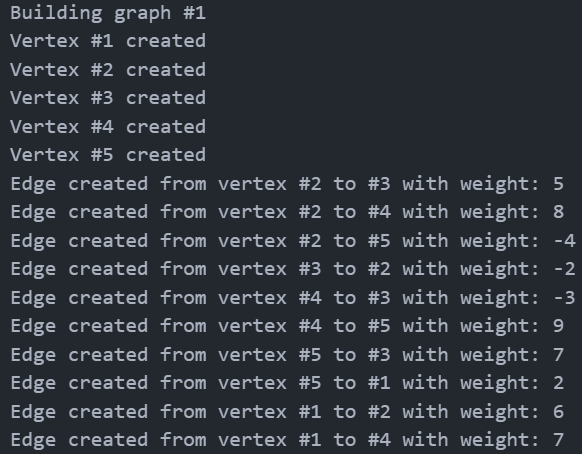
\includegraphics{images/Graph1_ParseBuild.png}
\end{center}
Here we see that, for \textbf{Graph 1}, five vertices are created and ten edges are created between the vertices.
Each characterized by some weight.

\subsection{Single Source Shortest Path Algorithm} \label{Graph_SSSP}
After the graph is built, using the first vertex returned by the build function, a Single Source Shortest Path algorithm is ran.
This algorithm calculates the path of least cost from some source to every available sink.
It does this by performing every possible traversal from the source to every possible sink.
While doing this it keeps track of the most efficient, lest costly, path.
Once all pathways are traversed, and the best routes calculated, the program displays these shortest paths.

\subsubsection{Implementation}
\begin{center}
   \lstinputlisting[language=C++, caption=SSSP Implementation, firstline=221, lastline=268]{graph/DirectedGraph.h}
\end{center}
In the above code we see that mapPathways takes in some starting vertex ID and searches for the vertex.
Once found, its distance is set to 0, since it's the source.
Then for every other vertex, the path from the source to that vertex is calculated.
If that path is shorter than the existing path to that vertex, it is updated.
Then once all vertices have been mapped a check is ran to see if all shortest paths were mapped.
Finally the result is output along with the path taken to get from the source to that sink.
\vspace*{5px}
\newline
The below function is a helper-function for outputting the shortest path:
\begin{center}
   \lstinputlisting[language=C++, caption=SSSP Helper, firstline=48, lastline=57]{graph/DirectedGraph.h}
\end{center}
This uses recursion to take the path of the most efficient route from sink to source and reorder it in reverse to get the correct path displayed.
Resulting in a path from source to sink, instead of backwards.

\subsubsection{Results}
\begin{center}
   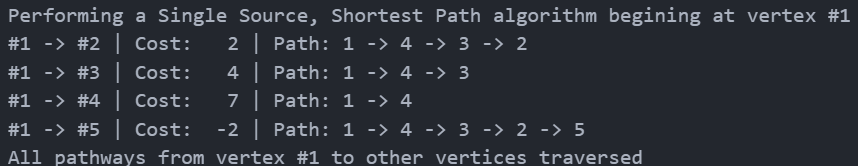
\includegraphics{results/Graph1_SSSP.png}
\end{center}
Here we see that the SSSP was successful in calculating the shortest path, path of least cost, between the first vertex, \textbf{\#1}, to the other four vertices.
Lastly, after comparing my results to those provided for \textbf{Graph 1}, no errors were found, meaning the algorithm ran properly.

\section{Spices \& Knapsacks} \label{SpiceKnapsack}
The remaining workload of \textbf{Assignment 4} consists of creating certain spices and knapsacks.
Each spice is characteristics by a color, some total price, and a quantity.
The unit price for a spice is also calculated.
A knapsack is characterized simply as some number, describing the capacity of the knapsack.
\vspace*{5px}
\newline
To fulfill this we must:
\begin{itemize}
   \item Read and parse the spices and knapsacks in \texttt{spices.txt}
   \item Build all spices with their respective characteristics
   \item Build all knapsacks with their respective capacities
   \item Perform a fractional knapsack algorithm for each knapsack on all spices
   \item Destroy all knapsacks and spices and allocate memory
\end{itemize}

\subsection{Parsing \& Building} \label{SpiceKnapsack_ParseBuild}
The input file \texttt{spices.txt}, being so similarly formatted to \texttt{graph2.txt}, requires some of the same logic as before too.
However, unlike before, \texttt{spices.txt} does not have one instruction per line.
Instead, the line containing the spice characteristics contains multiple instruction, one per characteristic.
This results in an increase in complexity as when parsing a spice, we must parse each instruction on the line, instead of just the whole line.
\vspace*{5px}
\newline
To achieve this, I broke my logic into two main sections, parsing the whole of \texttt{spice.txt}, and parsing a specific line into its individual instructions.
This allows for reduced complexity and an easier overall time understanding the code.

\subsubsection{Implementation}
\begin{center}
   \lstinputlisting[language=C++, caption=Parsing File Implementation, firstline=55, lastline=78]{Parse.h}
\end{center}
Above consists of half of the parsing for the spices and knapsacks.
Again, the file is open and read, each line is parsed, comments skipped, and the vector of instructions is returned.
Breaking the file down in this way allowed me to make parsing the characteristics more dynamic as well.
\begin{center}
   \lstinputlisting[language=C++, caption=Parsing Instruction Implementation, firstline=80, lastline=114]{Parse.h}
\end{center}
The parseLine function handles breaking down an instruction into its commands.
It does that by taking a line and breaking it into chunks separated by ';'.
Then, since each chunk consists of the type and the value (separated by '='), only the data after '=' is kept.
This is done by reading each character in the line, and once it reaches a '=' it pushes the characters back to a string until stopping at ';'.
Then it is pushed back to the vector of strings.
After each subcommand in the instruction is separated, it returns this vector of commands.
\vspace*{5px}
\newline
Below we have the build functions which constructs the spices, with their defined characteristics, and the knapsacks, with their specified size.
The buildSpices function takes in all the instructions and the container for all the spices.
Then, using only instructions beginning with 'spice', it breaks the spice command into its subcommands and adds a spice, created within addSpice, to the spices container.
\begin{center}
   \lstinputlisting[language=C++, caption=Building Spices Implementation, firstline=60, lastline=76]{Build.h}
\end{center}
Next the knapsacks are built.
Just like before, all instructions and the knapsack container are passed in.
The instructions starting with 'knapsack' are broke down to just its data after the '=', using parseLine.
Then the knapsack, created within the addKnapsack function, is added to the knapsack container, converting the string command to an int for the size.
\begin{center}
   \lstinputlisting[language=C++, caption=Building Knapsacks Implementation, firstline=78, lastline=94]{Build.h}
\end{center}

\subsubsection{Results}
As we can see in the image below, all four spices from \texttt{spice.txt} were parsed and built correctly, with each spice's characteristics displayed too.
Also, all five knapsacks were constructed with their respective size as an integer, parsed and built from strings in the file.
\begin{center}
   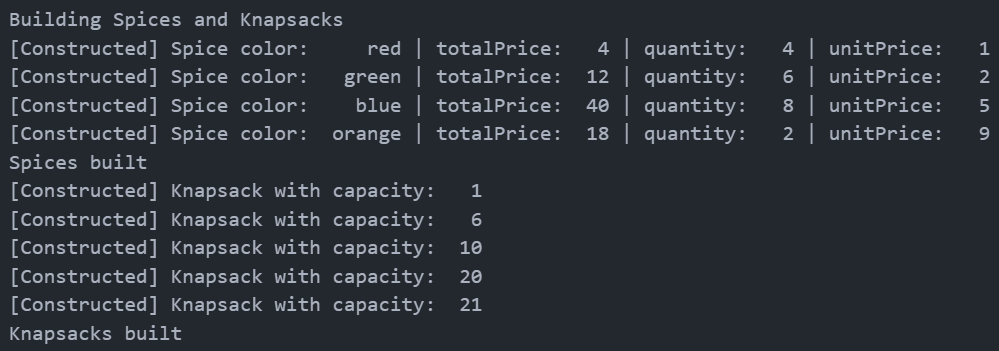
\includegraphics{images/SpiceKnapsack_ParseBuild.png}
\end{center}

\subsection{Fractional Knapsack Algorithm} \label{SpiceKnapsack_FKA}
Now that the spices and knapsacks have been successfully parsed and built, each knapsack is to be filled with spice.
This is done by using the fractional knapsack greedy algorithm.
Unlike the 0-1 knapsack problem, where only whole amounts of spice are allowed, fractional knapsack allows for percentages of spice.
0-1 knapsack is not solvable using a greedy algorithm, so dynamic programming is a necessity; fractional knapsack can be solved greedily and not dynamically.
\subsubsection{Implementation}
Building out the logic for fractional knapsack took some time.
The first step to having a working algorithm is properly ordering the spices in its container.
Using the my selection sort implementation from \textbf{Assignment 1}, with some small modifications, I reordered the spices by their unit price.
Then, starting with the most valuable spice, each spice is put in the knapsack until either the spice is gone, or the knapsack is full.
\begin{center}
   \lstinputlisting[language=C++, caption=Fractional Knapsack Implementation, firstline=79, lastline=111]{spice/SpiceKnapsack.h}
\end{center}
The function fillKnapsack takes in the knapsack to be filled, fills it, and reports its contents.
It does this by tracking the remaining space in the knapsack and filling the knapsack with the whole of a spice only if it will all fit.
Then for the remaining space it will take a fraction of spice to fill the space.
If the remaining space could not be filled by a fraction, it is also reported.
This is performed on every knapsack.

\subsubsection{Results}
Below are two filled knapsacks.
I've chosen these two knapsacks because they represent the two main challenges in this section.
Firstly, the knapsack with a capacity of 1.
This knapsack is too small for any one spice quantity so only a fractional quantity will fit.
As we see below, when this knapsack is filled, it can only store half of the orange spice.
Since orange costs 9 per quantity, and since we can only store one, the knapsack is filled and worth 9.
\begin{center}
   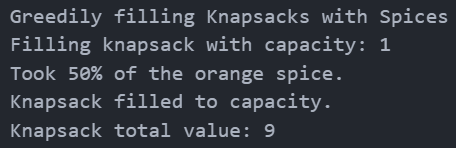
\includegraphics{results/SpiceKnapsack_Knapsack1_FracKnapsack.png}
\end{center}
Second, the knapsack with a capacity of 21.
This knapsack is too big for all the spice.
In total there are 20 units of spice, and since this is within the bounds of the knapsack, all spices are put in.
However, there is still more room in the sack, so the remaining space is recorded along with the contents and value of the knapsack.
\begin{center}
   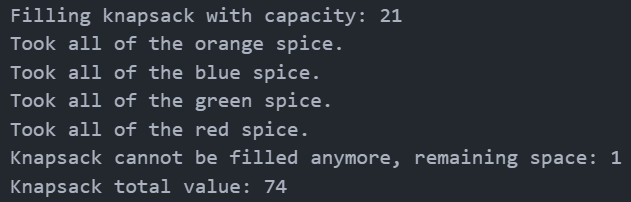
\includegraphics{results/SpiceKnapsack_Knapsack21_FracKnapsack.png}
\end{center}

\section{Clean Up} \label{CleanUp}
After each graph is built and the SSSP calculated, it is automatically rewritten with the next graph.
Once all graphs have been realized, the spices and knapsacks are parsed and constructed.
Then the fractional knapsack greedy algorithm is performed.
Finally, when everything has finished running, the destructors are called and the modified graph, the spices, and the knapsacks are destroyed.
\begin{center}
   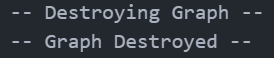
\includegraphics{images/Graph_Destruction.png}
\end{center}
Above we see that the graph is destroyed successfully, below we see that after the knapsacks are filled, the knapsacks are destroyed, then the spices.
\begin{center}
   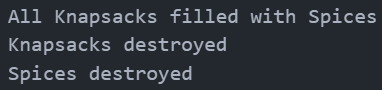
\includegraphics{images/SpiceKnapsack_CleanUp.png}
\end{center}
These destructor calls finish my program and completely clean up the memory accessed and modified in my code.
\vspace*{5px}
\newline
The remaining sections of this document describe the various functions and class structures used to complete this assignment that were not explicitly mentioned prior.

\section{Miscellaneous Implementations} \label{MiscImp}
\subsection{Main}
The \underline{main} file in my program consists of three functions.
The main function which houses the two function calls for graphing and for the spices and knapsacks operations.
And the two other functions, each consisting of the order in which parsing, building, and operating on the data is defined.
\begin{center}
   \lstinputlisting[language=C++, caption=Main Implementation, firstline=9, lastline=50]{Main.cpp}
\end{center}
The \underline{DirectedGraph} file houses the \textbf{Graph} class.
Each graph consists of a vector of vertices and a vector of edges.
A vertex contains an id, a processed flag, its distance to the single source, the predecessor vertex, and all neighboring vertices.
\begin{center}
   \lstinputlisting[language=C++, caption=Vertex Implementation, firstline=10, lastline=26]{graph/DirectedGraph.h}
\end{center}
An edge contains the starting and ending vertices's IDs as well as some weight or cost.
\begin{center}
   \lstinputlisting[language=C++, caption=Edge Implementation, firstline=27, lastline=40]{graph/DirectedGraph.h}
\end{center}
The \underline{SpiceKnapsack} file houses the classes for a \textbf{Spice} and a \textbf{Knapsack}.
A spice is characterized by some color, the total price of the spice, and the quantity of the spice.
Using the price and quantity, the total unit price can be derived.
\begin{center}
   \lstinputlisting[language=C++, caption=Spice Implementation, firstline=10, lastline=26]{spice/SpiceKnapsack.h}
\end{center}
A knapsack is defined as simply an integer representing its size.
\begin{center}
   \lstinputlisting[language=C++, caption=Knapsack Implementation, firstline=46, lastline=56]{spice/SpiceKnapsack.h}
\end{center}
For all results, see the figures folder in this directory.
In it you will find an images folder, containing the data parsed, and a results folder, containing the results from the operations performed on the data.

\end{document}
